\documentclass[11pt,letterpaper]{article}
\usepackage[margin=2cm]{geometry}
\usepackage{amsmath,amssymb,graphicx,xcolor,booktabs,tabularx,enumitem,titlesec,fancyhdr,array,longtable,caption}
\usepackage{tikz}
\usetikzlibrary{arrows.meta,positioning,shapes.geometric,calc}
\usepackage[hidelinks]{hyperref}
\usepackage{helvet}\renewcommand{\familydefault}{\sfdefault}
\usepackage{microtype}
\titleformat{\section}{\Large\bfseries\color{blue!50!black}}{\thesection}{0.6em}{}
\titleformat{\subsection}{\large\bfseries}{\thesubsection}{0.6em}{}
\titleformat{\subsubsection}{\normalsize\bfseries\color{blue!40!black}}{}{0em}{}
\setlength{\headheight}{14pt}
\pagestyle{fancy}\fancyhf{}\lhead{sPHENIX Self-Paced Course}\rhead{Module 2: RHIC and detector}\cfoot{\thepage}
\setlist{itemsep=1pt,topsep=3pt}
\setlength{\emergencystretch}{3em}
\setlength{\parskip}{3pt}
\newcommand{\conceptbox}[2]{\par\medskip\noindent\fcolorbox{blue!50!black}{blue!5}{\begin{minipage}{0.96\linewidth}\textbf{#1}\par\smallskip #2\end{minipage}}\par\medskip}
\newcommand{\connectbox}[1]{\par\medskip\noindent\fcolorbox{green!40!black}{green!6}{\begin{minipage}{0.96\linewidth}\textbf{Connect to your analysis.}\par\smallskip #1\end{minipage}}\par\medskip}
\newcommand{\pitfallbox}[1]{\par\medskip\noindent\fcolorbox{red!50!black}{red!4}{\begin{minipage}{0.96\linewidth}\textbf{Pitfalls.}\par\smallskip #1\end{minipage}}\par\medskip}
\newcommand{\checksbox}[1]{\par\medskip\noindent\fcolorbox{orange!60!black}{orange!6}{\begin{minipage}{0.96\linewidth}\textbf{Checks.}\par\smallskip #1\end{minipage}}\par\medskip}
\newcommand{\goal}[1]{\noindent\textbf{Goal.} #1\par}
\newcommand{\sqs}{\sqrt{s_{_{NN}}}}
\newcommand{\pT}{p_{\mathrm{T}}}
\newcommand{\RAA}{R_{AA}}
\begin{document}
\begin{center}
{\LARGE\bfseries sPHENIX Self-Paced Course}\\[4pt]
{\Large Module 2: RHIC and the sPHENIX detector:\\ layout, global detectors, runs and centrality}\\[8pt]
Prepared for P.\,D.\ Lewis (Ohio University) \quad November 2026\\[2pt]
\small Self-contained study text based on the Summer-2026 sPHENIX School and Workfest (BNL), public sPHENIX papers, the coresoftware source and standard accelerator and detector physics
\end{center}

\tableofcontents
\newpage

\section*{How to use this module}
\addcontentsline{toc}{section}{How to use this module}
This module is self-contained: you can learn everything here by reading it, without slides, recordings or papers.
It starts from the accelerator (how beams are made, focused, bunched, polarized and collided), goes through the layout of
the detector and its coordinate system, then explains the global detectors (MBD, ZDC, sEPD) and the three event-level
quantities they provide: the collision vertex, the centrality and the event plane. It ends with the collision systems
and runs of 2023--2025. The school talks below are listed only as the sources the text paraphrases, cited as [S\#\#].
Read once straight through, then answer the self-test questions (Section~\ref{sec:selftest}) before reading
Appendix~\ref{app:answers}. Exercises are optional; the text does not depend on them.

\subsection*{Learning objectives}
\begin{enumerate}[label=O\arabic*.]
\item Describe the RHIC injector chain and rings, and compute beam rigidity, revolution frequency and bunch spacing.
\item Explain bunches, the beam clock, crossing angle, luminous region, luminosity and pile-up, with numbers.
\item Explain how proton polarization is preserved (spin tune, resonances, Siberian snakes) and how it is measured (pC and H-jet polarimeters).
\item Draw the sPHENIX layout in $r$--$z$, state the coverage of each subsystem, and use the sPHENIX coordinate system.
\item Explain the MBD, ZDC and sEPD: technology, acceptance, signals, and the coresoftware objects that carry their output.
\item Explain how the vertex, the centrality (with Glauber modelling) and the event plane (with resolution corrections) are obtained.
\item Summarise the collision systems and runs 2023--2025 and why each was taken.
\end{enumerate}
\textbf{Prerequisites:} Module 1 (kinematics, $\RAA$, flow). \textbf{Estimated time:} 9--10 hours.

\noindent\textbf{School talks used as sources} (all ``sPHENIX School 2026'', BNL, July--August 2026):
\begin{itemize}
\item {[S01]} J.\ Huang, M.\ Connors, ``Welcome to sPHENIX school and sPHENIX Overview''.
\item {[S08]} J.\ Haggerty, ``HCal and Global Detector Overview''.
\item {[S48]} K.\ Hock, ``Spin dynamics at the RHIC accelerator complex (workfest lecture)''.
\item {[S49]} X.\ Chu, ``Polarimetry at RHIC (workfest lecture)''.
\item {[S05]} M.\ Mitrankova, R.\ Belmont, ``Bulk TG Analysis Opportunities''.
\item Supporting: {[S02]} D.\ Morrison, ``sPHENIX History''; {[S07]} J.\ Putschke, Y.\ Go, ``Jet Structure TG Analysis Opportunities''.
\end{itemize}
\textbf{Public readings} (optional): Glauber review \cite{glauber}; RHIC ZDC paper \cite{zdc}; flow methods \cite{pv};
the sPHENIX proposal \cite{proposal}; the first sPHENIX papers \cite{bulk1,bulk2,dijet,isogamma}.

\section{The RHIC accelerator complex}\label{sec:rhic}
\goal{Know how a RHIC beam is produced and stored, and compute its basic parameters.}

\subsection{The chain}
RHIC consists of two independent superconducting storage rings, called \emph{Blue} and \emph{Yellow}, in a tunnel of
3.834 km circumference. They cross at six interaction regions named after the positions on a clock; sPHENIX sits at IR8
(``8 o'clock''), the former PHENIX hall, and STAR at IR6 [S48]. Beams are prepared in a chain of injectors:
\begin{itemize}
\item \textbf{Polarized protons}: the optically pumped polarized ion source (OPPIS) makes polarized H$^-$ ions; a 200 MeV
linac accelerates them; the Booster (to about 2.5 GeV) and the AGS (to about 24 GeV) follow; the AtR transfer line injects into
RHIC, which accelerates to the store energy (100 GeV for $\sqrt s=200$ GeV) [S48].
\item \textbf{Heavy ions} (Au, O): an ion source and pre-accelerator feed the Booster and AGS, with stripping of electrons
along the way, before injection into RHIC.
\end{itemize}
In OPPIS, a laser polarizes electrons of rubidium atoms in a magnetic field; protons pick up polarized electrons;
a field-reversal region (a Sona transition) transfers the polarization from the electron to the proton; a second electron
is then added to make H$^-$ for the linac [S48].

\subsection{Beam optics in one page}
\textbf{Bending.} A particle of momentum $p$ and charge $q$ in a field $B$ moves on a circle of radius $\rho$ with
\begin{equation}
B\rho=\frac{p}{q},\qquad B\rho\,[\mathrm{T\,m}]=\frac{p\,[\mathrm{GeV}/c]}{0.2998\,Z}.
\end{equation}
The quantity $B\rho$ is the \emph{rigidity}. A 100 GeV proton has $B\rho=334$ T\,m. A gold nucleus at 100 GeV per nucleon has
$p\approx197\times100$ GeV and $Z=79$, so $B\rho\approx832$ T\,m: gold needs about 2.5 times stronger fields than protons at
the same energy per nucleon. This is why RHIC's top energy per nucleon is lower for gold than for protons.

\textbf{Focusing.} Quadrupoles focus in one transverse plane and defocus in the other; alternating them (FODO cells) gives net
focusing in both. Transverse motion obeys Hill's equation $y''+K(s)y=0$, with solution
$y(s)=\sqrt{\varepsilon\beta(s)}\cos(\phi(s)+\phi_0)$ [S48]. Here $\varepsilon$ is the emittance (phase-space area/$\pi$, an
invariant of the motion), $\beta(s)$ the beta function set by the magnets, and the number of betatron oscillations per turn
is the \emph{tune} $\nu=\frac{1}{2\pi}\oint ds/\beta(s)$. The rms beam size is $\sigma=\sqrt{\varepsilon\beta}$. At the
interaction point the final-focus quadrupoles make $\beta$ small ($\beta^*$) to squeeze the beam and raise luminosity.
Tunes must avoid resonances (simple fractions) where small field errors add up turn after turn.

\subsection{Bunches and the beam clock}
The radio-frequency (RF) system groups particles into bunches. Each ring has 120 bunch positions (``crossings'') around
the circumference; in the sPHENIX spin database the number of crossings is a constant 120 (\texttt{SpinDBContent::GetNCrossing()}).
Some positions are left empty as an abort gap, so typically about 110 bunches are filled. The numbers follow from the circumference:
\begin{align}
f_{\rm rev}&=c/C=299\,792\,458/3833.8\ \mathrm{Hz}\approx78.2\ \mathrm{kHz},\\
f_{\rm bunch}&=120\,f_{\rm rev}\approx9.38\ \mathrm{MHz},\qquad \Delta t=1/f_{\rm bunch}\approx106.6\ \mathrm{ns}.
\end{align}
This is the ``beam clock'' of the experiment: about 9.4 million possible bunch crossings per second [S08]. The sPHENIX
calorimeter and MBD waveform digitizers sample at six times this frequency, about 56.3 MHz [S08], i.e.\ six samples per
crossing, which is what makes waveform fitting (Module 7) possible.

\textbf{Satellite bunches.} The storage RF of RHIC also defines finer buckets about 5 ns apart. A small fraction of the
beam can sit in neighbouring buckets (satellites); collisions of a satellite with a main bunch are displaced in time by
$\sim5$ ns and in $z$ by $c\,\Delta t/2\approx76$ cm. The coresoftware class \texttt{MinimumBiasClassifier} assigns events to
a main, $-5$ ns or $+5$ ns ``bunch class'' from the corrected MBD $t_0$ (see the comments in \texttt{MinimumBiasClassifier.h}).

\subsection{Luminosity, crossing angle and pile-up}
For two Gaussian bunches colliding head-on with $N_1,N_2$ particles, $n_b$ bunches and transverse sizes $\sigma_x,\sigma_y$
(equal for the two beams),
\begin{equation}
\mathcal L=\frac{f_{\rm rev}\,n_b\,N_1N_2}{4\pi\sigma_x\sigma_y}.
\label{eq:lumi}
\end{equation}
\textbf{Toy numbers.} $N=2\times10^{11}$, $n_b=111$, $\sigma=150\ \mu$m: $\mathcal L\approx1.2\times10^{32}$ cm$^{-2}$s$^{-1}$
(these are illustrative, not measured RHIC values). The event rate of a process is $R=\sigma\mathcal L$; the integrated
luminosity is $\int\mathcal L\,dt$, with $1\ \mathrm{pb}^{-1}=10^{36}$ cm$^{-2}$, so $10^{31}$ cm$^{-2}$s$^{-1}$ for $10^5$ s gives 1 pb$^{-1}$.

\textbf{Vernier scans.} Eq.~(\ref{eq:lumi}) cannot be evaluated precisely from beam instrumentation alone. In a Vernier
(van der Meer) scan the beams are moved across each other in $x$ and $y$; the rate of a reference trigger (for example MBD
north-and-south coincidences) versus separation is a Gaussian of width $\Sigma=\sqrt{\sigma_1^2+\sigma_2^2}$. The scan gives
$\Sigma_x,\Sigma_y$ and hence the absolute luminosity at zero separation,
$\mathcal L=f_{\rm rev}\sum_b N_{1b}N_{2b}/(2\pi\Sigma_x\Sigma_y)$, and so the cross section seen by the reference trigger,
$\sigma_{\rm ref}=R_{\rm max}/\mathcal L$. Afterwards the luminosity of any run follows from the reference-trigger scaler
counts divided by $\sigma_{\rm ref}$ (corrected for pile-up and vertex acceptance). Module 9 treats this in detail.

\textbf{Crossing angle.} RHIC bunches are long (tens of cm rms) compared with the silicon trackers' acceptance of about
$|z|<10$ cm. With a head-on collision the luminous region has rms length $\sigma_z/\sqrt2$. Colliding at a full crossing angle
$\phi$ shortens it, to first approximation
\begin{equation}
\sigma_{z,\rm lum}\approx\frac{\sigma_z/\sqrt2}{\sqrt{1+\left(\sigma_z\tan(\phi/2)/\sigma_x\right)^2}},
\end{equation}
and reduces the luminosity by the same factor. Toy numbers: $\sigma_z=40$ cm, $\sigma_x=150\ \mu$m. Head-on: 28 cm;
$\phi=1$ mrad: 17 cm; $\phi=2$ mrad: 10 cm. sPHENIX runs with a 2 mrad crossing angle precisely to concentrate collisions
in $|z|<10$ cm for the silicon trackers [S08]. The MBD vertex distribution measured during a crossing-angle scan shows the
luminous region narrowing as the angle grows [S08]; this is a direct, visible check of the machine.

\textbf{Pile-up.} The mean number of interactions per filled crossing is $\mu=\sigma_{\rm inel}\mathcal L/(n_bf_{\rm rev})$.
Toy: $\sigma_{\rm inel}^{pp}\approx42$ mb and $\mathcal L=2\times10^{31}$ cm$^{-2}$s$^{-1}$ give $R=0.84$ MHz and
$\mu\approx0.10$. With Poisson statistics, the fraction of crossings with at least one collision that contain two or more is
$\approx\mu/2\approx5\%$. Calorimeters integrate over one crossing; the TPC drift (tens of $\mu$s) integrates over hundreds
of crossings, which is why tracking pile-up must be handled by time association (Module 4).

\connectbox{For your cross section, $\mathcal L$ comes from GL1 scalers of the MB trigger (bit 10) divided by its visible
cross section, with a pile-up correction that grows with $\mu$; the MB trigger itself is the MBD coincidence. The 2 mrad
crossing angle also matters for you: it narrows the $z$ distribution, which reduces the fraction of events lost to a
$|z_{\rm vtx}|$ cut and changes the photon acceptance through the vertex dependence of cluster $\eta$ (Section~\ref{sec:vertex}).}

\section{Polarized protons: spin dynamics and polarimetry}\label{sec:spin}
\goal{Understand how RHIC keeps protons polarized up to 100 GeV and how the polarization used in every spin analysis is measured [S48,S49].}

\subsection{Spin precession and the spin tune}
A magnetic moment in a field feels a torque $\vec\Gamma\propto\vec S\times\vec B$. In a ring the spin precesses around the
vertical bending field faster than the momentum turns; the motion is described by the Thomas--BMT equation
\begin{equation}
\frac{d\vec S}{dt}=\frac{q}{\gamma m}\vec S\times\left[(1+G\gamma)\vec B_\perp+(1+G)\vec B_\parallel\right]\quad(\text{electric terms neglected}),
\end{equation}
where $G=1.7928$ is the proton's anomalous magnetic moment [S48]. Relative to the momentum, the spin makes $\nu_s=G\gamma$
turns per revolution: the \emph{spin tune}. At injection into RHIC ($G\gamma=45.5$, about 24 GeV) and at 100 GeV ($G\gamma\approx191$)
the spin precesses hundreds of times faster than the orbit bends.

\subsection{Depolarizing resonances}
A small horizontal field kick tilts the spin. If kicks repeat in phase with the spin precession, they add up and depolarize
the beam [S48]. Two families exist:
\begin{itemize}
\item \textbf{Imperfection resonances}, $G\gamma=n$ (integer), driven by orbit errors (misalignments); they act on all particles equally.
\item \textbf{Intrinsic resonances}, $G\gamma=kP\pm\nu_y$ ($P$ the superperiodicity, $\nu_y$ the vertical tune), driven by betatron
oscillations in quadrupoles; their strength grows with the particle's betatron amplitude, i.e.\ with emittance.
\end{itemize}
Crossing an isolated resonance of strength $\epsilon_K$ at rate $\alpha=dG\gamma/d\theta$ leaves
$P_f/P_i=2e^{-\pi|\epsilon_K|^2/(2\alpha)}-1$ (Froissart--Stora): fast crossing preserves polarization, slow crossing of a
strong resonance flips it fully [S48]. Larger emittance (needed for more intensity) means stronger intrinsic resonances for the
large-amplitude particles; polarization and luminosity therefore compete in the injectors [S48].

\subsection{Siberian snakes}
A \emph{Siberian snake} is a set of helical dipoles that rotates the spin by 180$^\circ$ about a horizontal axis without
disturbing the orbit much. Two full snakes on opposite sides of a ring, with axes $90^\circ$ apart, make the spin tune
$\nu_s=1/2$ independent of energy, so resonance conditions are never met during acceleration [S48]. RHIC has two full snakes
per ring (four helical dipoles each); the AGS has two partial snakes that rotate the spin by less than 180$^\circ$ and open a
gap in the spin tune; horizontal ``tune jumps'' in the AGS cross the remaining weak horizontal resonances quickly [S48].
Even with snakes, the betatron tunes must stay in a narrow window below 0.7 (to avoid the 7/10 snake resonance) and away
from $2/3$ (a strong betatron resonance), while the beam--beam interaction spreads the tunes [S48].

\subsection{Spin direction at the experiment}
The stable spin direction in RHIC is vertical. Spin rotators around IR6 and IR8 can turn it into the horizontal plane for
longitudinal running [S48]. sPHENIX ran with transverse (vertical) polarization in 2024 and 2025. Bunches are filled with
alternating spin patterns (up/down sequences that differ between Blue and Yellow and between fills), so both spin states
are collected simultaneously and slow detector drifts cancel.

\subsection{Polarimetry}
The beam polarization is $P=\epsilon/A_N$: measure a left--right asymmetry $\epsilon=(N_L-N_R)/(N_L+N_R)$ of a reaction with known
analyzing power $A_N$ [S49]. RHIC uses two kinds of polarimeters.
\begin{itemize}
\item \textbf{Proton--carbon (pC) polarimeters}: two per ring (four in total) [S49]. An ultra-thin carbon ribbon is moved
through the beam; recoil carbon nuclei from elastic scattering in the Coulomb--nuclear interference (CNI) region are detected in
silicon strip detectors (six detectors of twelve strips each) [S49]. Each measurement takes minutes and is repeated
several times per fill; scanning the ribbon also measures the polarization profile across the beam. The carbon energy is
calibrated with an $^{241}$Am $\alpha$ source (5.486 MeV); the energy lost in the detector's dead layer and the timing offset
are fitted from the correlation of energy and time of flight (the ``banana'' band) [S49]. The $A_N$ of pC scattering is not
known precisely from theory, so pC gives only a \emph{relative} polarization.
\item \textbf{Hydrogen-jet (H-jet) polarimeter}: a polarized atomic hydrogen gas jet crosses both beams. Because the reaction
is $pp$ elastic scattering, the same $A_N$ applies whether the beam or the target is polarized:
$\epsilon_{\rm beam}=A_NP_{\rm beam}$ and $\epsilon_{\rm target}=A_NP_{\rm target}$, so
$P_{\rm beam}=P_{\rm target}\,\epsilon_{\rm beam}/\epsilon_{\rm target}$, with $P_{\rm target}$ measured independently.
No knowledge of $A_N$ is needed. It is slow (about one absolute measurement per fill) but precise [S49].
\end{itemize}
\textbf{Combination.} The pC values are normalized to the H-jet: $P_{\rm beam}=C\cdot P_{\rm pC}^{\rm rel}$ with
$C=P^{\rm abs}_{\rm HJ}/P^{\rm HJ}_{\rm pC}$, where $P^{\rm HJ}_{\rm pC}$ is the pC average over the fills used by the H-jet [S49].
Further corrections: the beam polarization profile (the experiment sees the luminosity-weighted average, not the
pC-scanned one), polarization decay during a fill ($dP/dt$), and spin-tilt corrections if the stable spin direction is not
exactly vertical. Systematic uncertainties include H-jet molecular-hydrogen contamination and background, the pC scale and
fill-to-fill uncertainty, and the profile correction [S49]. The polarimetry group provides final fill-by-fill values and
uncertainties for each run; analyses must use those official values, with the prescribed way to compute run- or
fill-averaged polarization [S49].

\checksbox{Blue and Yellow polarizations are separate numbers per fill. A spin analysis that combines beams must weight by
each beam's polarization. Local polarimetry in the experiment (for example forward-neutron asymmetries in the ZDC shower-maximum
detector, as in PHENIX) confirms the spin direction at IR8; a non-zero radial or longitudinal component would show up there.}

\pitfallbox{Using per-measurement polarimeter numbers rather than the final fill-averaged values; forgetting the overall
polarization scale uncertainty, which is fully correlated between all points of an $A_N$ measurement; mixing up which ring
goes towards $+z$ at IR8 (take it from the spin analysis documentation, not from memory).}

\section{The sPHENIX detector layout and coordinates}\label{sec:layout}
\goal{Be able to draw the detector from memory, know what each layer does, and use the coordinate system correctly.}

\subsection{Layout}
sPHENIX is a barrel detector built around the former BaBar superconducting solenoid, operated at 1.4 T
[S02]. From the beam outwards (Figure~\ref{fig:layout}):
\begin{enumerate}
\item \textbf{MVTX}: three layers of monolithic active pixel sensors (MAPS) a few cm from the beam; precise vertexing and
displaced-vertex tagging.
\item \textbf{INTT}: a barrel of silicon strip ladders at intermediate radius (inner and outer ladder layers, 56 ladders in total); single-crossing timing,
which tags the bunch crossing of a track \cite{intt1,intt2}.
\item \textbf{TPC}: a compact time projection chamber from about 20 to 78 cm radius; momentum measurement.
\item \textbf{TPOT}: micromegas modules just outside the TPC, for TPC distortion calibration.
\item \textbf{EMCal}: tungsten-powder/scintillating-fibre (SPACAL) towers, 24\,576 towers in a $96\times256$ $(\eta,\phi)$ grid,
$|\eta|<1.1$, about 18 radiation lengths deep [S08] \cite{calo}.
\item \textbf{Inner HCal}: mostly aluminium with scintillating tiles, inside the solenoid (radius about 1.16--1.37 m) [S08].
\item \textbf{Solenoid}: about 1.4 radiation lengths of material between inner and outer HCal [S08].
\item \textbf{Outer HCal}: tilted steel plates with scintillating tiles, outside the solenoid (radius about 1.9--2.6 m); the steel is
the magnet's flux return. 32 sectors, 1536 towers of $\Delta\eta\times\Delta\phi\approx0.1\times0.1$, five tiles per tower
(7680 tiles), about 3.5 interaction lengths [S08].
\item \textbf{Global detectors} at forward rapidity: MBD ($z=\pm2.53$ m), sEPD (just outside the barrel ends), ZDC ($\pm18$ m).
\end{enumerate}
The inner and outer HCal have the same $24\times64$ tower segmentation, so towers can be combined; together with the EMCal
they absorb most of the energy of jets up to several tens of GeV [S08]. Module 3 covers the calorimeters and Module 4 the trackers.

\begin{figure}[h]\centering
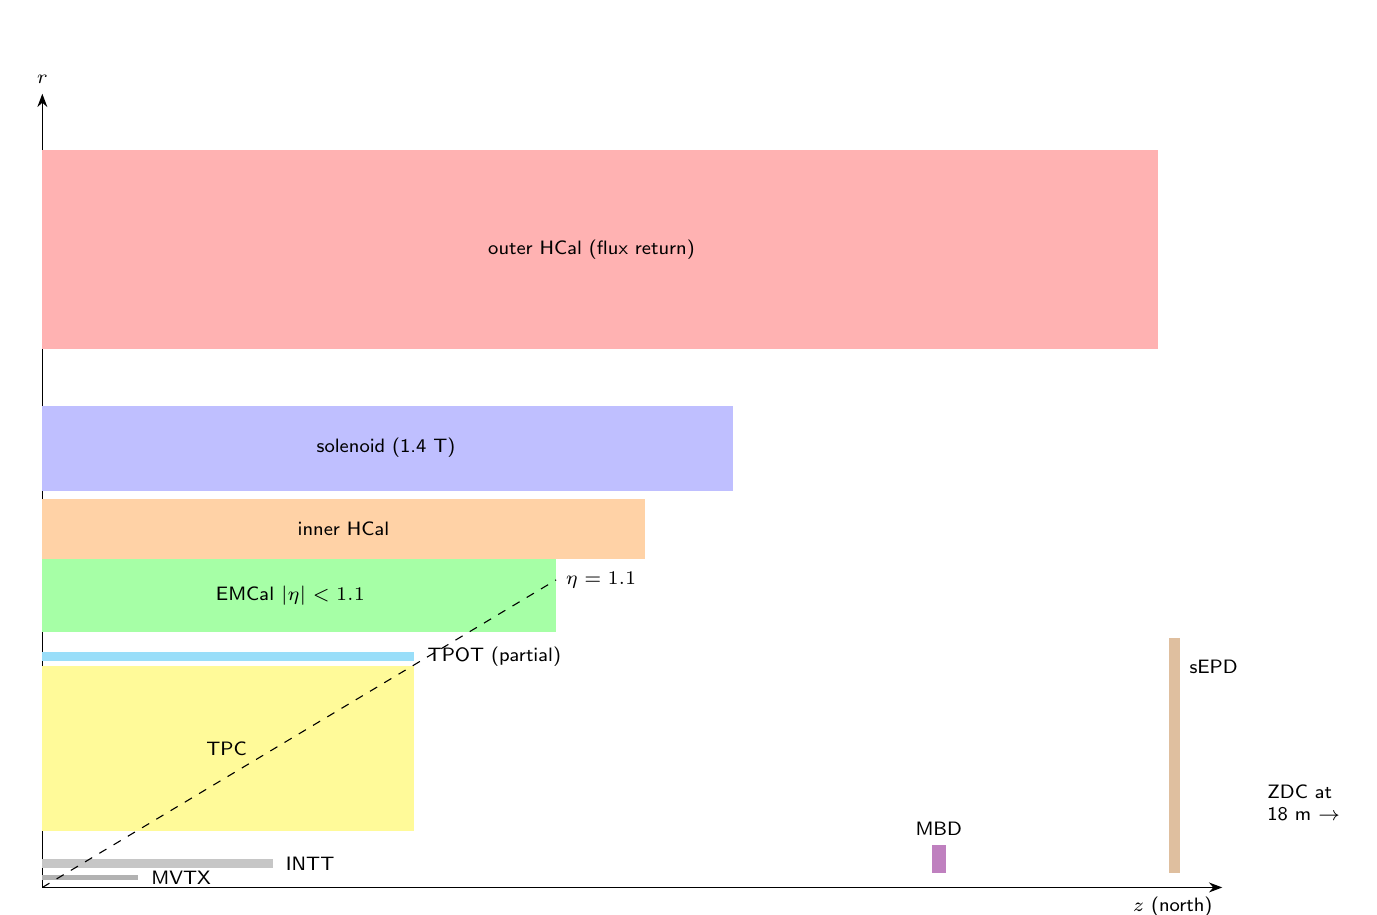
\begin{tikzpicture}[x=0.45cm,y=0.36cm,font=\scriptsize]
% r-z quarter view: z horizontal (0..28 -> 0..280 cm scale 10cm/unit), r vertical (0..27 units -> 0..270 cm)
\draw[-{Stealth}] (0,0)--(33.3,0) node[below left]{$z$ (north)};
\draw[-{Stealth}] (0,0)--(0,28) node[above]{$r$};
\fill[gray!60] (0,0.25) rectangle (2.7,0.45); \node[right] at (2.8,0.35){MVTX};
\fill[gray!45] (0,0.7) rectangle (6.5,1.0); \node[right] at (6.6,0.85){INTT};
\fill[yellow!40] (0,2.0) rectangle (10.5,7.8); \node at (5.2,4.9){TPC};
\fill[cyan!40] (0,8.0) rectangle (10.5,8.3); \node[right] at (10.6,8.15){TPOT (partial)};
\fill[green!35] (0,9.0) rectangle (14.5,11.6); \node at (7,10.3){EMCal $|\eta|<1.1$};
\fill[orange!35] (0,11.6) rectangle (17,13.7); \node at (8.5,12.65){inner HCal};
\fill[blue!25] (0,14.0) rectangle (19.5,17.0); \node at (9.7,15.5){solenoid (1.4 T)};
\fill[red!30] (0,19.0) rectangle (31.5,26.0); \node at (15.5,22.5){outer HCal (flux return)};
\fill[violet!50] (25.1,0.5) rectangle (25.5,1.5); \node[above] at (25.3,1.5){MBD};
\fill[brown!50] (31.8,0.5) rectangle (32.1,8.8); \node[right] at (32.1,7.8){sEPD};
\draw[dashed] (0,0)--(14.5,10.85) node[pos=1.0,right]{$\eta=1.1$};
\node[align=left] at (35.6,3.0){ZDC at\\ 18 m $\rightarrow$};
\end{tikzpicture}
\caption{Schematic $r$--$z$ quarter view of sPHENIX (north half, $z>0$). Approximate radii and lengths only; not to scale for
the outer HCal ends, the sEPD and the ZDC. Check the sPHENIX detector paper or the Geant4 geometry for exact dimensions.}
\label{fig:layout}\end{figure}


\subsection{Granularity, and what it means for photons}
The EMCal grid of $96\times256$ towers over $|\eta|<1.1$ and $2\pi$ gives $\Delta\eta=2.2/96=0.023$ and
$\Delta\phi=2\pi/256=0.0245$ rad per tower. At a radius of about 93 cm a tower face is therefore about 2.3 cm wide. The HCal
($24\times64$) has $\Delta\eta\approx0.092$ and $\Delta\phi=0.098$, so one HCal tower sits behind roughly $4\times4$ EMCal
towers. This 4:1 mapping is used by the calorimeter triggers and by jet reconstruction with ``retowered'' EMCal energy.

\textbf{Photon-pair separation.} A $\pi^0$ of energy $E$ decays into two photons whose minimum opening angle is
$\psi_{\rm min}\approx2m_{\pi^0}/E$ (symmetric decay). In units of EMCal towers at $\eta\approx0$:
\begin{center}\small
\begin{tabular}{@{}lccccc@{}}\toprule
$E$ (GeV) & 2 & 5 & 10 & 15 & 20\\\midrule
$\psi_{\rm min}$ (rad) & 0.135 & 0.054 & 0.027 & 0.018 & 0.0135\\
$\psi_{\rm min}$ (towers) & 5.5 & 2.2 & 1.1 & 0.73 & 0.55\\\bottomrule
\end{tabular}\end{center}
Above about 10 GeV the two showers (each several towers wide, Module 3) overlap strongly and the clusterizer often merges
them into one cluster. For the $\eta$ meson ($m=0.548$ GeV) the same separation is reached at about four times higher energy.
This is why $\pi^0$ reconstruction by pairing two clusters loses efficiency at high $\pT$, and why shower-shape
discrimination or merged-cluster techniques are needed there.

\subsection{Subsystem summary}
\begin{table}[h]\centering\small
\begin{tabularx}{\linewidth}{@{}lXXl@{}}\toprule
Subsystem & Technology & Main role & coresoftware package\\\midrule
MVTX & 3 layers of MAPS pixels & primary and secondary vertices, DCA & \texttt{mvtx}\\
INTT & silicon strips, 56 ladders & bunch-crossing tag, seeding & \texttt{intt}\\
TPC & gas TPC with GEM readout & momentum, $dE/dx$ & \texttt{tpc}, \texttt{tpccalib}\\
TPOT & micromegas & TPC distortion calibration & \texttt{micromegas}\\
EMCal & W-powder/SciFi SPACAL, SiPM & photons, electrons, $\pi^0$, jets & \texttt{CaloBase}, \texttt{CaloReco}\\
iHCal / oHCal & Al or steel + scint.\ tiles, SiPM & hadronic energy, jets & \texttt{CaloBase}, \texttt{CaloReco}\\
MBD & quartz Cherenkov + PMTs & MB trigger, vertex, $t_0$, centrality & \texttt{mbd}\\
sEPD & scint.\ tiles + SiPM & event plane, centrality & \texttt{epd}, \texttt{eventplaneinfo}\\
ZDC & W/fibre calorimeter + SMD & spectator neutrons, luminosity & \texttt{zdcinfo}\\
\bottomrule\end{tabularx}
\caption{sPHENIX subsystems. Event-level products: \texttt{globalvertex}, \texttt{centrality}, \texttt{trigger}, \texttt{uspin}.}
\end{table}

\subsection{Coordinate system}
\begin{itemize}
\item $z$ along the beam axis, origin at the nominal interaction point; $+z$ points \textbf{north}. In the MBD code arm 0 is
south ($z=-253$ cm) and arm 1 is north ($z=+253$ cm) (\texttt{MbdGeomV1.cc}).
\item $y$ vertically up; $x$ horizontal, completing a right-handed system (with $+z$ north and $+y$ up this makes $+x$ point west).
\item $\phi$ is the azimuth around $z$ measured from $+x$; $\theta$ the polar angle from $+z$; $\eta=-\ln\tan(\theta/2)$.
\item Calorimeter towers are labelled by integer $\eta$ and $\phi$ bins packed into a 32-bit key; use the functions in
\texttt{TowerInfoDefs} (package \texttt{CaloBase}) to decode keys rather than assuming a numbering. Check there how bin 0 maps to
$\eta$ and $\phi$ before using raw indices.
\end{itemize}
Physical cluster positions are in cm in this frame. A cluster's $\eta$ is computed with respect to a vertex: with respect to
$z=0$ it is a \emph{detector} $\eta$; with respect to the event vertex it is the \emph{physics} $\eta$. Many bugs come from
mixing the two (Section~\ref{sec:vertex}).

\subsection{The solenoid and momentum measurement}
A charged particle in the solenoid's axial field follows a helix with transverse radius $R$:
\begin{equation}
\pT\,[\mathrm{GeV}]=0.3\,B\,[\mathrm T]\,R\,[\mathrm m].
\end{equation}
At 1.4 T, a 1 GeV track has $R=2.38$ m. Over a lever arm $L$ the sagitta is $s=L^2/(8R)$; across the TPC (from 0.2 to 0.78 m,
$L=0.58$ m) it is 17.7 mm at 1 GeV, 3.5 mm at 5 GeV. Since $\delta\pT/\pT=\delta s/s\propto\pT$, momentum resolution degrades
linearly with $\pT$ at high $\pT$; this, and the need to separate $\Upsilon$ states, set the TPC point resolution requirements.
Low-$\pT$ tracks curl up: a track needs $\pT\gtrsim0.3\times1.4\times0.39\approx0.16$ GeV to reach the TPC outer radius ($2R>0.78$ m).
For the EMCal at about 0.9 m radius, tracks below about 0.2 GeV never reach it.

\section{The global detectors}\label{sec:global}
\goal{Know what the MBD, ZDC and sEPD are made of, what they measure, and where their output lives in the software [S08].}

\subsection{Minimum Bias Detector (MBD)}
\textbf{Hardware.} The MBD is the PHENIX beam--beam counter (BBC), reused [S08]. Each arm has 64 photomultiplier tubes
(PMTs) with quartz Cherenkov radiators on their faces (\texttt{MBD\_N\_PMT = 128} in \texttt{MbdDefs.h}). The arms sit at
$z=\pm253$ cm and cover about $3.5<|\eta|<4.6$, i.e.\ radii of roughly 5--15 cm from the beam [S08]. The PMTs are mesh-dynode
types that work in the fringe field of the solenoid. Quartz has refractive index 1.4585 (in \texttt{MbdDefs.h}), so a charged
particle radiates Cherenkov light only if $\beta>1/n=0.686$; slow particles and neutral particles do not fire it directly.

\textbf{Electronics.} The PMT signals are split in front-end modules into a channel optimized for charge and one optimized for
timing; the shaped signals are digitized by sPHENIX waveform digitizers and recorded by the DAQ [S08]. A cost-effective
timing design gives a single-channel time resolution of a few tens of picoseconds [S08].

\textbf{Charge calibration.} A single minimum-ionizing particle (MIP) through one radiator produces a Landau-shaped charge
spectrum; the most probable value sets the gain of each PMT. The calibrated charge per arm is then a count of charged particles
(in MIP units), which is the input to centrality and to the event plane [S08].

\textbf{Time and vertex.} For each arm the arrival time is taken from the PMTs above about a quarter of the MIP peak: a
Gaussian fit around the \emph{earliest} cluster of PMT times, which suppresses late secondaries [S08]. With $t_S$ and $t_N$
the south and north times,
\begin{equation}
z_{\rm vtx}=\frac{c\,(t_S-t_N)}{2},\qquad t_0=\frac{t_S+t_N}{2}\ (\text{after subtracting the flight time } 253\ \mathrm{cm}/c\approx8.44\ \mathrm{ns}).
\label{eq:mbdz}
\end{equation}
This is exactly what \texttt{MbdEvent.cc} computes (arm 0 south, arm 1 north). \textbf{Numbers:} a time difference of 0.67 ns
corresponds to 10 cm; a 0.5 ns difference to 7.5 cm. A collision at positive $z$ is closer to the north arm, so $t_N<t_S$ and
$z>0$. If the per-arm time is the average of $N$ hit PMTs each with resolution $\sigma_t$, the vertex resolution is about
$c\,\sigma_t/(\sqrt2\sqrt N)$: better in central Au+Au (many hits) than in $p$+$p$ (few hits).

\textbf{Trigger.} The MBD samples every one of the $\sim9.4$ million crossings per second and selects collisions with high
efficiency for inelastic Au+Au events; Au+Au collision rates of 50 kHz or more were possible [S08]. Trigger conditions
combine a minimum number of hits in both arms (north AND south) with optional vertex windows. In $p$+$p$ the MBD sees only
part of the inelastic cross section; that part is the trigger's visible cross section, which the Vernier scan measures.

\textbf{Software.} Package \texttt{mbd}: \texttt{MbdReco} (a SubsysReco) builds \texttt{MbdPmtContainer} (per-PMT charge and
time) and \texttt{MbdOut}, with \texttt{get\_zvtx()}, \texttt{get\_t0()}, \texttt{get\_q(arm)}, \texttt{get\_npmt(arm)} and
\texttt{get\_time(arm)}. The vertex is also stored as an \texttt{MbdVertex} in an \texttt{MbdVertexMap} (package
\texttt{globalvertex}); calibrations are in \texttt{MbdCalib}.

\subsection{Zero Degree Calorimeters (ZDC)}
\textbf{Hardware.} Identical ZDCs were built for all RHIC experiments \cite{zdc}. Each side has three modules of about two
nuclear interaction lengths each (tungsten absorber sampled by optical fibres that collect Cherenkov light), located about 18 m
from the interaction point behind the DX dipole magnets [S08]. The DX magnets sweep charged particles away, so the ZDC sees
neutral particles within about 2 mrad of the beam: mostly spectator neutrons from the colliding nuclei \cite{zdc}.
A shower-maximum detector (SMD) of scintillator strips between the first and second modules measures the transverse position
of the neutron shower [S08]. The sPHENIX ZDC reuses the PHENIX detectors with new instrumentation (analog sums for triggers and
digitized waveforms) [S08].

\textbf{Uses.} (1) Event characterization: the spectator-neutron energy anti-correlates with MBD charge in central collisions;
together they separate central from very peripheral events, and help identify pile-up. (2) Luminosity monitoring and Vernier
scans: north--south coincidences are a standard luminosity reference at RHIC \cite{zdc}. (3) Energy scale: in Au+Au the
single-neutron peak (about 100 GeV, from mutual Coulomb dissociation) calibrates the ZDC. (4) Local polarimetry in $p$+$p$ and
ultra-peripheral collision tagging via forward neutrons. (5) Spectator reaction plane from the SMD.

\textbf{Software.} Package \texttt{zdcinfo}: \texttt{ZdcReco} fills \texttt{Zdcinfo} with \texttt{get\_zdc\_energy(arm)},
\texttt{get\_radius(arm)} (from the SMD position) and \texttt{get\_zvertex()} (from ZDC timing).

\subsection{sPHENIX Event Plane Detector (sEPD)}
\textbf{Hardware.} Two wheels (north and south) of scintillator tiles covering $2.0<|\eta|<4.9$ [S05], segmented in rings of
$\eta$ and sectors of $\phi$, following the design of the STAR Event Plane Detector. In total there are 744 channels
(\texttt{SEPD\_CHANNELS = 744} in \texttt{EventPlaneReco.h}); tiles are addressed by arm, sector and tile id
(\texttt{EPDDefs.h}). Light from wavelength-shifting fibres embedded in each tile is carried by clear fibres to SiPMs; the
readout electronics were adapted from the EMCal electronics [S08]. Early tests used cosmic rays to see clean MIP peaks per
tile [S08]. The sEPD was funded by NSF through Lehigh [S02].

\textbf{Uses.} Event planes for harmonics $n=2,3,4$ (the harmonics in \texttt{EventPlaneReco}); an alternative centrality
estimator (\texttt{CentralityInfo} has \texttt{epd\_N}, \texttt{epd\_S}, \texttt{epd\_NS} entries next to the MBD ones);
forward multiplicity. The large gap between the sEPD and the barrel suppresses non-flow correlations.

\subsection{Beam-background counters}
Small scintillator counters (``inner'' and ``outer donuts'' around the beam pipe, and ``collars'') monitor beam-related
background such as beam--gas interactions and halo; their discriminated signals go to the RHIC scalers so the accelerator
operators can tune the beams [S08].

\checksbox{(1) MBD $z$ vs.\ track vertex $z$: a tight diagonal with a slope of one; a constant offset means a timing calibration
problem. (2) MBD north vs.\ south charge: correlated, symmetric for symmetric systems. (3) ZDC vs.\ MBD charge in Au+Au: the
characteristic ``boomerang'' (spectator neutrons rise from central to mid-central, then fall in peripheral events where
neutrons are bound in fragments). (4) sEPD tile charge spectra: a clear MIP peak per tile.}

\pitfallbox{Taking $z_{\rm vtx}$ from the MBD in events where one arm has few hits (large tails); forgetting satellite-bunch
collisions displaced by about 76 cm; mixing MBD arm numbering (0 = south, 1 = north).}

\section{Vertexing}\label{sec:vertex}
\goal{Know the vertex sources available in sPHENIX, how they are combined, and how the vertex enters a calorimeter analysis.}

\subsection{Sources}
\begin{itemize}
\item \textbf{MBD vertex} (Eq.~\ref{eq:mbdz}): available in every MBD-triggered event, independent of tracking; resolution of
order a cm or better depending on multiplicity.
\item \textbf{Track vertex} (SVTX): fitted from reconstructed tracks (silicon seeds or full tracks); precise in $x$, $y$ and $z$,
and able to separate pile-up vertices in different crossings (with INTT timing). Requires the tracking chain (Module 8).
\item \textbf{Calorimeter vertex}: for calorimeter-only data the $z$ position can be estimated from calorimeter information alone;
the package \texttt{calovtxreco} contains several such algorithms (including machine-learning variants), stored as
\texttt{CaloVertex} objects. Treat these as specialized tools and read their documentation before use.
\end{itemize}
\textbf{GlobalVertexReco} (package \texttt{globalvertex}) collects the available vertices into a \texttt{GlobalVertexMap};
each \texttt{GlobalVertex} records which types it contains (\texttt{VTXTYPE}: \texttt{MBD}=300, \texttt{SVTX}=400,
\texttt{SVTX\_MBD}=500, \texttt{CALO}=250 and variants, \texttt{TRUTH}=100, among others). In an analysis you ask for the type you
want (for example with \texttt{find\_vertexes(GlobalVertex::MBD)}) and must handle events where it is missing.

\subsection{How the vertex enters a photon analysis}
A cluster at radius $r$ and longitudinal position $z_c$ has, relative to a vertex at $z_v$,
$\eta=\sinh^{-1}\!\left[(z_c-z_v)/r\right]$ and $E_T=E/\cosh\eta$. \textbf{Worked example.} A cluster at $r=93$ cm with
detector $\eta=0.5$ sits at $z_c=93\sinh0.5=48.5$ cm. If the true vertex is at $z_v=+10$ cm, the physics $\eta$ is
$\sinh^{-1}(38.5/93)=0.403$, and $E_T$ computed with $z_v=0$ is too small by the factor $\cosh0.403/\cosh0.5$, i.e.\ by 4\%.
For a spectrum falling as $\pT^{-8}$ that is up to about a 30\% effect on the yield at fixed $\pT$ if left uncorrected. The pair opening
angle, and hence the $\pi^0$ mass, also change with the vertex. A vertex cut ($|z|<10$, 30 or 60 cm depending on the analysis)
also limits how far the shower axis is from the tower axis (the EMCal towers are projective only approximately).

\connectbox{Your $p$+$p$ analysis uses the MBD vertex for every cluster. Three consequences: (1) the cluster $\eta$ and $E_T$
must be recomputed with $z_{\rm MBD}$, consistently in data and in PYTHIA8; (2) the simulated vertex distribution should be
reweighted to the data MBD $z$ distribution (the crossing angle shapes it); (3) events with no MBD vertex are lost, and this
inefficiency, together with the $|z|$ cut acceptance, is part of the luminosity normalization (the MB trigger cross section
is defined with a vertex condition). In Au+Au, the MBD vertex resolution is better because many PMTs fire.}

\section{Centrality and the Glauber model}\label{sec:cent}
\goal{Understand what centrality means, how it is measured with the MBD, and where $\langle N_{\rm part}\rangle$ and
$\langle N_{\rm coll}\rangle$ come from \cite{glauber}.}

\subsection{Geometry}
The impact parameter $b$ (the distance between the centres of the nuclei) is not measurable. Centrality classes are defined as
percentiles of the total inelastic cross section, ordered by a measured quantity that is monotonic in $b$ on average: 0--10\%
are the 10\% of events with the largest MBD charge, and so on.

\subsection{Glauber model}
\textbf{Nuclear density.} Nucleons are distributed according to a Woods--Saxon profile
$\rho(r)=\rho_0/[1+e^{(r-R)/a}]$; for gold the standard parameters are $R=6.38$ fm and $a=0.535$ fm \cite{glauber}.

\textbf{Monte Carlo Glauber.} (1) Sample nucleon positions for each nucleus; (2) pick $b$ from $d\sigma\propto2\pi b\,db$;
(3) treat nucleons as moving on straight lines; two nucleons collide if their transverse distance is below
$d=\sqrt{\sigma^{\rm inel}_{NN}/\pi}$. With $\sigma_{NN}^{\rm inel}\approx42$ mb $=4.2$ fm$^2$ at 200 GeV, $d=1.16$ fm.
(4) Count $N_{\rm part}$ (nucleons with at least one collision) and $N_{\rm coll}$ (all binary collisions). Repeating many times
gives the distributions of $N_{\rm part}$, $N_{\rm coll}$, $b$ and the eccentricities $\varepsilon_n$ used in Module 1.
The optical limit replaces sampling by the overlap function $T_{AB}(b)=\int d^2s\,T_A(\vec s)T_B(\vec s-\vec b)$, with
$\langle N_{\rm coll}\rangle=\sigma_{NN}T_{AB}$; the two approaches differ in detail, especially for fluctuations \cite{glauber}.

\subsection{From MBD charge to centrality}
\begin{enumerate}
\item Model the MBD charge as a sum over ``ancestors'' $N_{\rm anc}=fN_{\rm part}+(1-f)N_{\rm coll}$, each producing charge
according to a negative binomial distribution (NBD) with parameters $\mu,k$.
\item Fit the MBD charge-sum distribution in data, at high charge where the trigger is fully efficient, by varying $f,\mu,k$.
\item The ratio of data to fit at low charge gives the trigger efficiency; the MB trigger misses part of the most peripheral events.
\item Define centrality cuts on the charge such that each class contains the right fraction of the \emph{total} cross section
(including the part the trigger missed).
\item Map each class to $\langle N_{\rm part}\rangle$, $\langle N_{\rm coll}\rangle$, $\langle T_{AA}\rangle$ from the Glauber events in the same class.
\end{enumerate}
\textbf{In coresoftware:} \texttt{MinimumBiasClassifier} (package \texttt{trigger}) decides whether an event is minimum bias
(\texttt{MinimumBiasInfo::isAuAuMinimumBias()}, with species \texttt{AUAU}, \texttt{OO}, \texttt{PP}, pile-up rejection and bunch
classes); \texttt{CentralityReco} (package \texttt{centrality}) writes \texttt{CentralityInfo}, whose
\texttt{get\_centile(CentralityInfo::PROP::mbd\_NS)} returns the centrality percentile from the MBD north+south charge. The
division tables and vertex-dependent scale factors come from the conditions database.

\textbf{Systematics.} Varying the trigger efficiency within its uncertainty shifts the class boundaries and matters most for
peripheral classes. Varying the Glauber inputs ($\sigma_{NN}$, $R$, $a$, nucleon exclusion distance) changes
$\langle N_{\rm coll}\rangle$. For $R_{CP}$ part of this cancels in the ratio of central to peripheral $\langle N_{\rm coll}\rangle$.

\connectbox{Your M.S.\ $R_{CP}$ used exactly this chain: MBD centrality, Glauber $\langle N_{\rm coll}\rangle$ per class, and their
uncertainties. The peripheral normalization is the most fragile point because of the trigger inefficiency. Pile-up and
satellite collisions (Section~\ref{sec:rhic}) can move events between centrality classes, which is why the minimum-bias
classifier rejects them.}


\subsection{Centrality and impact parameter: a toy picture}
If every collision with $b<b_{\rm max}$ were inelastic (a sharp-cutoff ``black disc''), the centrality of an event with impact
parameter $b$ would be $c\approx\pi b^2/(\pi b_{\rm max}^2)=b^2/b_{\rm max}^2$. Toy: $b_{\rm max}\approx14.9$ fm for Au+Au gives a
total cross section of $\pi b_{\rm max}^2\approx7$ b and
\begin{center}\small
\begin{tabular}{@{}lcccccc@{}}\toprule
centrality $c$ & 5\% & 10\% & 20\% & 40\% & 60\% & 80\%\\\midrule
$b$ (fm) & 3.3 & 4.7 & 6.7 & 9.4 & 11.5 & 13.3\\\bottomrule
\end{tabular}\end{center}
The real relation is smeared: at fixed $b$, $N_{\rm part}$ and the MBD charge fluctuate, so a centrality class corresponds to a
\emph{distribution} of $b$. This smearing is largest in peripheral events and in small systems (O+O), where centrality selection
can also bias the hard-process yield (a high-$\pT$ process adds multiplicity, pushing the event into a more central class).

\subsection{Centrality in O+O and $p$+$p$}
For O+O the same machinery applies with an oxygen density profile (oxygen is light, so nucleon positions and correlations
matter more), and the MBD acceptance covers a smaller multiplicity. In $p$+$p$ there is no centrality; instead one uses
``event activity'' classes (for example MBD charge), with care because the selection correlates with the hard process.

\section{The event plane}\label{sec:ep}
\goal{Understand how the event-plane angle is estimated, corrected and resolution-corrected \cite{pv}.}

\subsection{Q-vectors}
For harmonic $n$ and detector elements $j$ (sEPD tiles or MBD PMTs) at azimuth $\phi_j$ with weight $w_j$ (charge),
\begin{equation}
Q_{n,x}=\sum_jw_j\cos n\phi_j,\quad Q_{n,y}=\sum_jw_j\sin n\phi_j,\quad \Psi_n=\frac1n\,\mathrm{atan2}(Q_{n,y},Q_{n,x}).
\end{equation}
\textbf{Corrections.} A real detector has non-uniform acceptance and gains, so $\Psi_n$ is not flat. \emph{Recentering}
subtracts the run- and centrality-averaged $\langle Q_n\rangle$ (and may rescale by its width). \emph{Flattening} (the shift
method) adds $\Delta\Psi_n=\sum_k\frac{2}{nk}\left[-\langle\sin nk\Psi_n\rangle\cos nk\Psi_n+\langle\cos nk\Psi_n\rangle\sin nk\Psi_n\right]$
so that the final distribution is flat. In coresoftware \texttt{EventPlaneReco} produces raw, recentered and shifted
$Q$-vectors and angles (\texttt{Eventplaneinfo::get\_qvector\_raw}, \texttt{get\_qvector\_recentered}, \texttt{get\_shifted\_psi}),
including per-ring $Q$-vectors, with calibrations from the conditions database.

\subsection{Resolution}
Because $\Psi_n$ is estimated from a finite number of particles, it fluctuates around the true symmetry plane, and
$v_n^{\rm obs}=\langle\cos n(\phi-\Psi_n)\rangle=v_n\,\mathcal R_n$ with $\mathcal R_n=\langle\cos n(\Psi_n-\Psi_n^{\rm true})\rangle<1$.
With two equivalent sub-events A and B (sEPD north and south),
\begin{equation}
\mathcal R_n^{\rm sub}=\sqrt{\langle\cos n(\Psi_n^A-\Psi_n^B)\rangle}.
\end{equation}
Toy: $\langle\cos2(\Psi_2^N-\Psi_2^S)\rangle=0.16$ gives $\mathcal R_2^{\rm sub}=0.40$; an observed $v_2^{\rm obs}=0.024$ measured
with one sub-event then corresponds to $v_2=0.06$. With three different detectors A, B, C (e.g.\ sEPD south, sEPD north, MBD)
the three-sub-event formula
$\mathcal R_A=\sqrt{\langle\cos n(\Psi_A-\Psi_B)\rangle\langle\cos n(\Psi_A-\Psi_C)\rangle/\langle\cos n(\Psi_B-\Psi_C)\rangle}$
gives each resolution separately \cite{pv}.

\checksbox{After flattening, $\Psi_n$ is flat within statistics in every centrality class and run. $\langle\cos n(\Psi^N-\Psi^S)\rangle$
is largest in mid-central events for $n=2$ (where $v_2$ and multiplicity are both sizeable). The resolution-corrected $v_n$ agrees
between event-plane detectors.}

\pitfallbox{Using a full-event resolution when the analysis uses a sub-event plane (or the reverse); calibrating recentering on one
run period and applying it to another; correlating particles with an event plane built from the same particles (auto-correlation)
--- the $\eta$ gap avoids it.}

\section{Collision systems and runs, 2023--2025}\label{sec:runs}
\goal{Know what data exist, why each system was taken, and the operational facts that affect analyses.}

\begin{table}[h]\centering\small
\begin{tabularx}{\linewidth}{@{}llX@{}}\toprule
Run & System ($\sqs=200$ GeV) & Purpose and notes\\\midrule
2023 & Au+Au & commissioning of all subsystems; first collisions at IR8 since PHENIX\\
2024 & $p^\uparrow$+$p^\uparrow$ & transversely polarized; a large calorimeter-triggered sample, a smaller all-subsystem sample and tracker streaming data; reference for heavy ions and the spin programme\\
2024 & Au+Au & the main QGP dataset with all subsystems; a field-off subset gave the first two physics papers \cite{bulk1,bulk2}\\
2025 & $p^\uparrow$+$p^\uparrow$ & with the upgraded DAQ, tracker streaming readout for most of the run; heavy-flavour baseline and spin measurements such as $D^0$ $A_N$\\
2025 & O+O & small-system QGP; direct comparison with LHC O+O\\
\bottomrule\end{tabularx}
\caption{sPHENIX collision systems [S01,S04,S07]. The 2025 run extended into early 2026 and ended on 6 February 2026, the last
RHIC run [S07,S08]. For integrated luminosities use the official collaboration tables, not numbers copied from talks.}
\label{tab:runs}\end{table}

\textbf{Why calorimeter-only data?} The TPC and MVTX cannot be read out for every MB-triggered crossing at the full collision rate in
triggered mode, while the calorimeters can be read out at a higher rate. Hence large ``calo-only'' samples for jets, photons
and neutral mesons, and smaller ``all-subsystem'' samples [S01,S04]. \textbf{Streaming readout} records the trackers continuously
rather than only on triggers, giving huge unbiased minimum-bias samples for heavy flavour and bulk physics; the 2025 DAQ buffer
upgrade made extensive streaming possible, including the first spin-polarized streaming collider data [S01]. sPHENIX recorded
the largest raw data volume of any RHIC experiment [S01]. Operations relied on hundreds of shifters and a run coordinator per
year who knows which runs are special [S01].


\subsection{Fills, stores and runs}
A RHIC \emph{fill} starts with injection of both rings, the energy ramp, and the squeeze to collision optics; the beams are
then brought into collision and the \emph{store} lasts several hours while the luminosity decays (intensity loss and emittance
growth) and, for protons, the polarization slowly decreases. The experiment records many \emph{runs} (each roughly up to an hour)
during a store; each run has a run number, a fixed trigger configuration and its own scaler record. The fill number links runs to
the polarimeter results and spin patterns. Conditions that change between fills (crossing angle, bunch intensities, beam
positions) change the vertex distribution and pile-up, which is why run-by-run QA is needed (Module 9).

\subsection{Beam backgrounds and empty bunches}
Not every recorded event is a beam--beam collision. Beam--gas interactions and beam halo hitting upstream material produce
showers, often entering the calorimeters at shallow angles, and cosmic rays cross the detector at random times. Two handles exist.
First, timing: beam--beam collisions have MBD hits in both arms with $t_0$ near zero, background does not. Second, the fill
pattern: in crossings where one ring's bunch is empty there are no beam--beam collisions, so triggers firing in those crossings
measure the beam-induced background per bunch. The GL1 bunch number and the fill pattern from the spin database give access to them.

\connectbox{Your Photon-3/4 triggered sample (bits 29/30) is the most exposed to non-collision background, because a single
energetic shower from beam halo can fire a photon trigger without an MBD coincidence. Requiring a valid MBD vertex removes most
of it; the residual can be estimated from triggers in empty-bunch crossings and from the cluster timing and shape.}

\textbf{Run-level information you will use.}
\begin{itemize}
\item \textbf{GL1} records per event the bunch number (\texttt{Gl1Packet::getBunchNumber()}), the live and scaled trigger
vectors (\texttt{getLiveVector()}, \texttt{getScaledVector()}) and scalers (\texttt{getScaler()}); \texttt{Gl1Packet} lives in
\texttt{offline/framework/ffarawobjects}. The helper \texttt{TriggerAnalyzer} (package \texttt{trigger}) offers
\texttt{didTriggerFire(name or bit)}, \texttt{getTriggerPrescale()}, \texttt{getTriggerScalers()},
\texttt{getTriggerLiveScalers()} and \texttt{getTriggerRawScalers()}.
\item \textbf{Spin database} (package \texttt{uspin}): \texttt{SpinDBOutput::GetDBContent(content, run)} fills a
\texttt{SpinDBContent} object. Its accessors include:
  \begin{itemize}
  \item \texttt{GetFillNumber()}, \texttt{GetCrossingShift()} (offset between the GL1 bunch number and the RHIC bucket);
  \item \texttt{GetSpinPatternBlue(bunch)} and \texttt{GetSpinPatternYellow(bunch)};
  \item \texttt{GetPolarizationBlue(...)} and \texttt{GetPolarizationYellow(...)};
  \item per-bunch scalers such as \texttt{GetScalerMbdVertexCut(bunch)} and \texttt{GetScalerZdcNoCut(bunch)};
  \item \texttt{GetBadBunchFlag(bunch)} and \texttt{GetCrossAngle()}.
  \end{itemize}
\item \textbf{DAQ and run databases} hold run type, duration, trigger configuration and scaledowns; find the current host names
and table names in the collaboration documentation.
\end{itemize}

\connectbox{For each run in your $p$+$p$ list you need: the MB (bit 10) and Photon (bits 29/30) scaledowns and live scalers from
GL1, the crossing angle (affects the vertex distribution), and the spin information only if you also do $A_N$. Runs with
anomalous crossing angles or MBD problems are candidates for exclusion in the good-run list (Module 9).}

\section{Hands-on exercises on SDCC (optional)}\label{sec:handson}
Suggestions only; they were not run while writing this text.
\begin{enumerate}
\item \textbf{Beam numbers.} Reproduce $f_{\rm rev}$, the 106.6 ns spacing, the 56.3 MHz sampling and the rigidities of
Section~\ref{sec:rhic} in a short ROOT or Python script.
\item \textbf{MBD vertex.} Write a SubsysReco (Module 6) or a ROOT macro on a DST that reads \texttt{MbdOut} and histograms
\texttt{get\_zvtx()}, \texttt{get\_t0()} and \texttt{get\_q(0)} vs \texttt{get\_q(1)}. Fit the $z$ distribution with a Gaussian
and compare its width with the toy crossing-angle formula.
\item \textbf{Spin DB.} In ROOT with the sPHENIX environment loaded, create a \texttt{SpinDBOutput}, call
\texttt{GetDBContent} for one of your runs and print the crossing angle, fill number, crossing shift and the first ten spin patterns.
\item \textbf{Scaledowns.} Use \texttt{TriggerAnalyzer} in a short module to print the prescale and the raw, live and scaled
scalers of bits 10, 29 and 30 for the first and last event of a segment.
\item \textbf{Toy Glauber.} Write a 100-line Monte Carlo Glauber for Au+Au (Woods--Saxon, $d=1.16$ fm) and compute
$\langle N_{\rm part}\rangle$ and $\langle N_{\rm coll}\rangle$ for $b<3$ fm and for $b=12$ fm.
\item \textbf{Checkpoint (syllabus).} Query the spin DB and DAQ DB for a run of your choice (crossing angle, scaledowns) and plot
the MBD vertex distribution for that run.
\end{enumerate}

\section{Self-test questions}\label{sec:selftest}
\begin{enumerate}[label=Q\arabic*.]
\item Compute the revolution frequency of RHIC and the bunch spacing. How many digitizer samples fit in one crossing?
\item Why does a gold beam at 100 GeV/nucleon need a larger $B\rho$ than a proton beam at 100 GeV?
\item What does the 2 mrad crossing angle buy sPHENIX, and what does it cost?
\item With $\mu=0.2$, what fraction of crossings with at least one collision have two or more?
\item What is a Vernier scan, and what quantity does it determine?
\item Why do Siberian snakes make the spin tune energy independent? What value does it take?
\item Why does the H-jet polarimeter not need to know $A_N$, while the pC polarimeter does?
\item The MBD measures $t_S=8.70$ ns and $t_N=8.20$ ns (after the same offsets). Where is the vertex?
\item Why does the MBD use quartz Cherenkov radiators rather than scintillator, and what is the velocity threshold?
\item What does the ZDC measure and why only neutral particles?
\item Describe how the MBD charge distribution is turned into centrality classes. Where does the trigger efficiency enter?
\item Compute the interaction distance $d$ for $\sigma_{NN}=42$ mb. What are $N_{\rm part}$ and $N_{\rm coll}$?
\item Two sub-event planes give $\langle\cos2(\Psi^N-\Psi^S)\rangle=0.09$. What is the sub-event resolution, and the true $v_2$ if $v_2^{\rm obs}=0.018$?
\item A cluster at $r=93$ cm has detector $\eta=0$. What is its physics $\eta$ for $z_v=-20$ cm, and by how much is $E_T$ changed?
\item Why does sPHENIX have both calorimeter-only and all-subsystem datasets?
\end{enumerate}

\section*{Glossary}
\addcontentsline{toc}{section}{Glossary}
\begin{description}[style=nextline,leftmargin=1.2cm,itemsep=0pt]
\item[Beam clock] 9.38 MHz bunch-crossing frequency; 120 crossings per turn.
\item[Blue / Yellow] the two RHIC rings.
\item[Crossing angle] angle between the beams at the IP; 2 mrad at sPHENIX.
\item[Emittance, $\beta^*$] phase-space size of the beam; beta function at the IP; $\sigma=\sqrt{\varepsilon\beta}$.
\item[GL1] global level-1 trigger; records trigger bits, scalers and bunch number.
\item[Glauber model] geometric model giving $N_{\rm part}$, $N_{\rm coll}$, $T_{AA}$ and $\varepsilon_n$.
\item[H-jet, pC] absolute and relative RHIC polarimeters.
\item[MBD] Minimum Bias Detector (ex-PHENIX BBC), quartz Cherenkov + PMTs at $z=\pm253$ cm.
\item[Pile-up] more than one collision in the same crossing (or detector integration time).
\item[Satellite bunch] beam in neighbouring RF buckets, giving collisions displaced by about 5 ns / 76 cm.
\item[sEPD] sPHENIX Event Plane Detector, $2.0<|\eta|<4.9$, 744 channels.
\item[Siberian snake] helical-dipole spin rotator that fixes the spin tune at 1/2.
\item[Spin tune] spin rotations per turn, $G\gamma$ without snakes.
\item[Vernier scan] beam-separation scan to measure the absolute luminosity.
\item[ZDC] Zero Degree Calorimeter at $\pm18$ m; spectator neutrons.
\end{description}

\begin{thebibliography}{99}
\bibitem{bulk1} sPHENIX Collaboration, Measurement of charged hadron multiplicity in Au+Au collisions at 200 GeV, JHEP 08 (2025) 075, arXiv:2504.02240.
\bibitem{bulk2} sPHENIX Collaboration, Measurement of the transverse energy density in Au+Au collisions at 200 GeV, Phys.\ Rev.\ C 112 (2025) 024908, arXiv:2504.02242.
\bibitem{dijet} sPHENIX Collaboration, Dijet transverse momentum imbalance and acoplanarity in $p$+$p$ collisions at 200 GeV, arXiv:2606.17184.
\bibitem{isogamma} sPHENIX Collaboration, Isolated prompt photon production in $p$+$p$ collisions at 200 GeV, arXiv:2607.03892.
\bibitem{intt1} sPHENIX INTT ladder and readout, Nucl.\ Instrum.\ Meth.\ A 1082 (2026) 171020, arXiv:2503.09105.
\bibitem{intt2} sPHENIX INTT test beam, Nucl.\ Instrum.\ Meth.\ A 1086 (2026) 171312, arXiv:2509.00908.
\bibitem{calo} C.\,A.\ Aidala et al., Design and beam test results for the sPHENIX electromagnetic and hadronic calorimeter prototypes, IEEE Trans.\ Nucl.\ Sci.\ 65 (2018) 2901--2919, arXiv:1704.01461.
\bibitem{proposal} PHENIX Collaboration, An Upgrade Proposal from the PHENIX Collaboration, arXiv:1501.06197.
\bibitem{roland} C.\ Roland for sPHENIX, sPHENIX experiment overview, EPJ Web Conf.\ 364, 01006 (2026).
\bibitem{glauber} M.\,L.\ Miller, K.\ Reygers, S.\,J.\ Sanders, P.\ Steinberg, Glauber modeling in high energy nuclear collisions, Ann.\ Rev.\ Nucl.\ Part.\ Sci.\ 57 (2007) 205, arXiv:nucl-ex/0701025.
\bibitem{zdc} C.\ Adler et al., The RHIC zero degree calorimeters, Nucl.\ Instrum.\ Meth.\ A 470 (2001) 488, arXiv:nucl-ex/0008005.
\bibitem{pv} A.\,M.\ Poskanzer and S.\,A.\ Voloshin, Methods for analyzing anisotropic flow in relativistic nuclear collisions, Phys.\ Rev.\ C 58 (1998) 1671, arXiv:nucl-ex/9805001.
\bibitem{pubpage} sPHENIX Public Results, \url{https://www.sphenix.bnl.gov/PublicResults}.
\end{thebibliography}
\noindent\textbf{School talks} (cited as [S\#\#]; Speaker, `Title', sPHENIX School 2026 (BNL, July 2026)):
[S01] J.\ Huang, M.\ Connors, `Welcome to sPHENIX school and sPHENIX Overview';
[S02] D.\ Morrison, `sPHENIX History';
[S04] G.\ Nukazuka, M.\ Sarsour, `Cold QCD TG Analysis Opportunities';
[S05] M.\ Mitrankova, R.\ Belmont, `Bulk TG Analysis Opportunities';
[S07] J.\ Putschke, Y.\ Go, `Jet Structure TG Analysis Opportunities';
[S08] J.\ Haggerty, `HCal and Global Detector Overview';
[S48] K.\ Hock, `Spin dynamics at the RHIC accelerator complex (workfest lecture)';
[S49] X.\ Chu, `Polarimetry at RHIC (workfest lecture)'.

\appendix
\section{Answers}\label{app:answers}
\begin{enumerate}[label=A\arabic*.]
\item $f_{\rm rev}=c/C=78.2$ kHz; $\Delta t=1/(120\times78.2\ \mathrm{kHz})=106.6$ ns; six samples at 56.3 MHz.
\item $B\rho=p/(Ze)$: gold carries 197 nucleons' momentum but only 79 charges, so $B\rho$ is $197/79\approx2.5$ times larger per unit
energy per nucleon (832 vs 334 T\,m).
\item It shortens the luminous region (toy: from 28 to 10 cm rms) so more collisions fall within the silicon acceptance $|z|<10$ cm;
it costs luminosity by the same geometric factor.
\item $P(\ge2)/P(\ge1)=(1-e^{-\mu}-\mu e^{-\mu})/(1-e^{-\mu})=(1-0.8187-0.1637)/0.1813=0.097$, about 10\%.
\item The beams are scanned across each other; the rate vs separation gives the overlap widths $\Sigma_x,\Sigma_y$, hence the absolute
luminosity and the visible cross section of the reference trigger.
\item Two full snakes with orthogonal axes make the one-turn spin rotation independent of $G\gamma$, with spin tune 1/2, so
resonance conditions are never satisfied during the ramp.
\item The H-jet uses the same elastic reaction with beam or target polarized; the ratio of asymmetries equals the ratio of
polarizations, and $P_{\rm target}$ is known. The pC $A_N$ comes from theory and is not precise, so pC is normalized to the H-jet.
\item $z=c(t_S-t_N)/2=29.98\times0.50/2=7.5$ cm, on the north side ($z>0$).
\item Cherenkov light is prompt (excellent timing) and has a velocity threshold that suppresses slow background; quartz is
radiation hard. Threshold $\beta>1/1.4585=0.686$.
\item Neutral energy (mostly spectator neutrons) within about 2 mrad of the beam, because the DX magnets sweep charged particles away.
\item Fit the charge distribution with Glauber+NBD at high charge; the deficit at low charge gives the trigger efficiency; cuts are
placed so that classes contain fixed fractions of the full cross section, including the missed fraction; each class is mapped to
Glauber averages.
\item $d=\sqrt{4.2/\pi}=1.16$ fm. $N_{\rm part}$: nucleons with at least one collision; $N_{\rm coll}$: total number of binary collisions.
\item $\mathcal R^{\rm sub}=\sqrt{0.09}=0.30$; $v_2=0.018/0.30=0.06$.
\item $z_c=0$, so the physics $\eta=\sinh^{-1}(20/93)=0.213$; $E_T$ is multiplied by $1/\cosh0.213=0.978$ (a 2.3\% decrease relative to the $z_v=0$ value).
\item The calorimeters can be read at higher rate than the TPC/MVTX in triggered mode; large calo-only samples serve jets, photons
and neutral mesons, while all-subsystem and streaming samples serve tracking-based physics.
\end{enumerate}
\end{document}
